\chapter{Theory}
\label{chap:theory}

The \acf{SM} of particle physics provides an extremely successful description of all known particles and interactions. Developed in the 1960s and 70s, the \ac{SM} has survived decades of experimental tests, predicting particles before their discovery and withstanding high precision tests. However, there are several known shortcomings of the \ac{SM} that lead physicists to believe that nature must deviate from the \ac{SM} at higher energies than currently experimentally accessible. 

One attractive extension to the \ac{SM} is \acf{SUSY}, which adds an additional symmetry to the \ac{SM} between fermions and bosons, creating an additional spectrum of particles that provides solutions to the open questions in the \ac{SM}. The particular \ac{SUSY} model probed by this thesis is \acf{GMSB} \ac{SUSY}. This chapter gives an overview of the \ac{SM} and the motivation and formulation of \ac{SUSY}, it then describes \ac{GMSB} models and their current experimental context. 


\section{The Standard Model}

The \acf{SM} provides a framework for all known particles and interactions through Quantum Field Theory (QFT). All known matter particles and force carriers are described through its formulation, as is the Higgs boson. The particles of the Standard Model are divided into fermions, leptons and quarks, with spin-$\frac{1}{2}$, and bosons with integer spin. Matter is made of fermions and forces are mediated through spin-1 bosons, the spin-0 Higgs boson gives mass to the fermions and other bosons. The particle content of the \ac{SM} is shown in \autoref{fig:sm}. 
 
\begin{figure}[htbp]
\centering
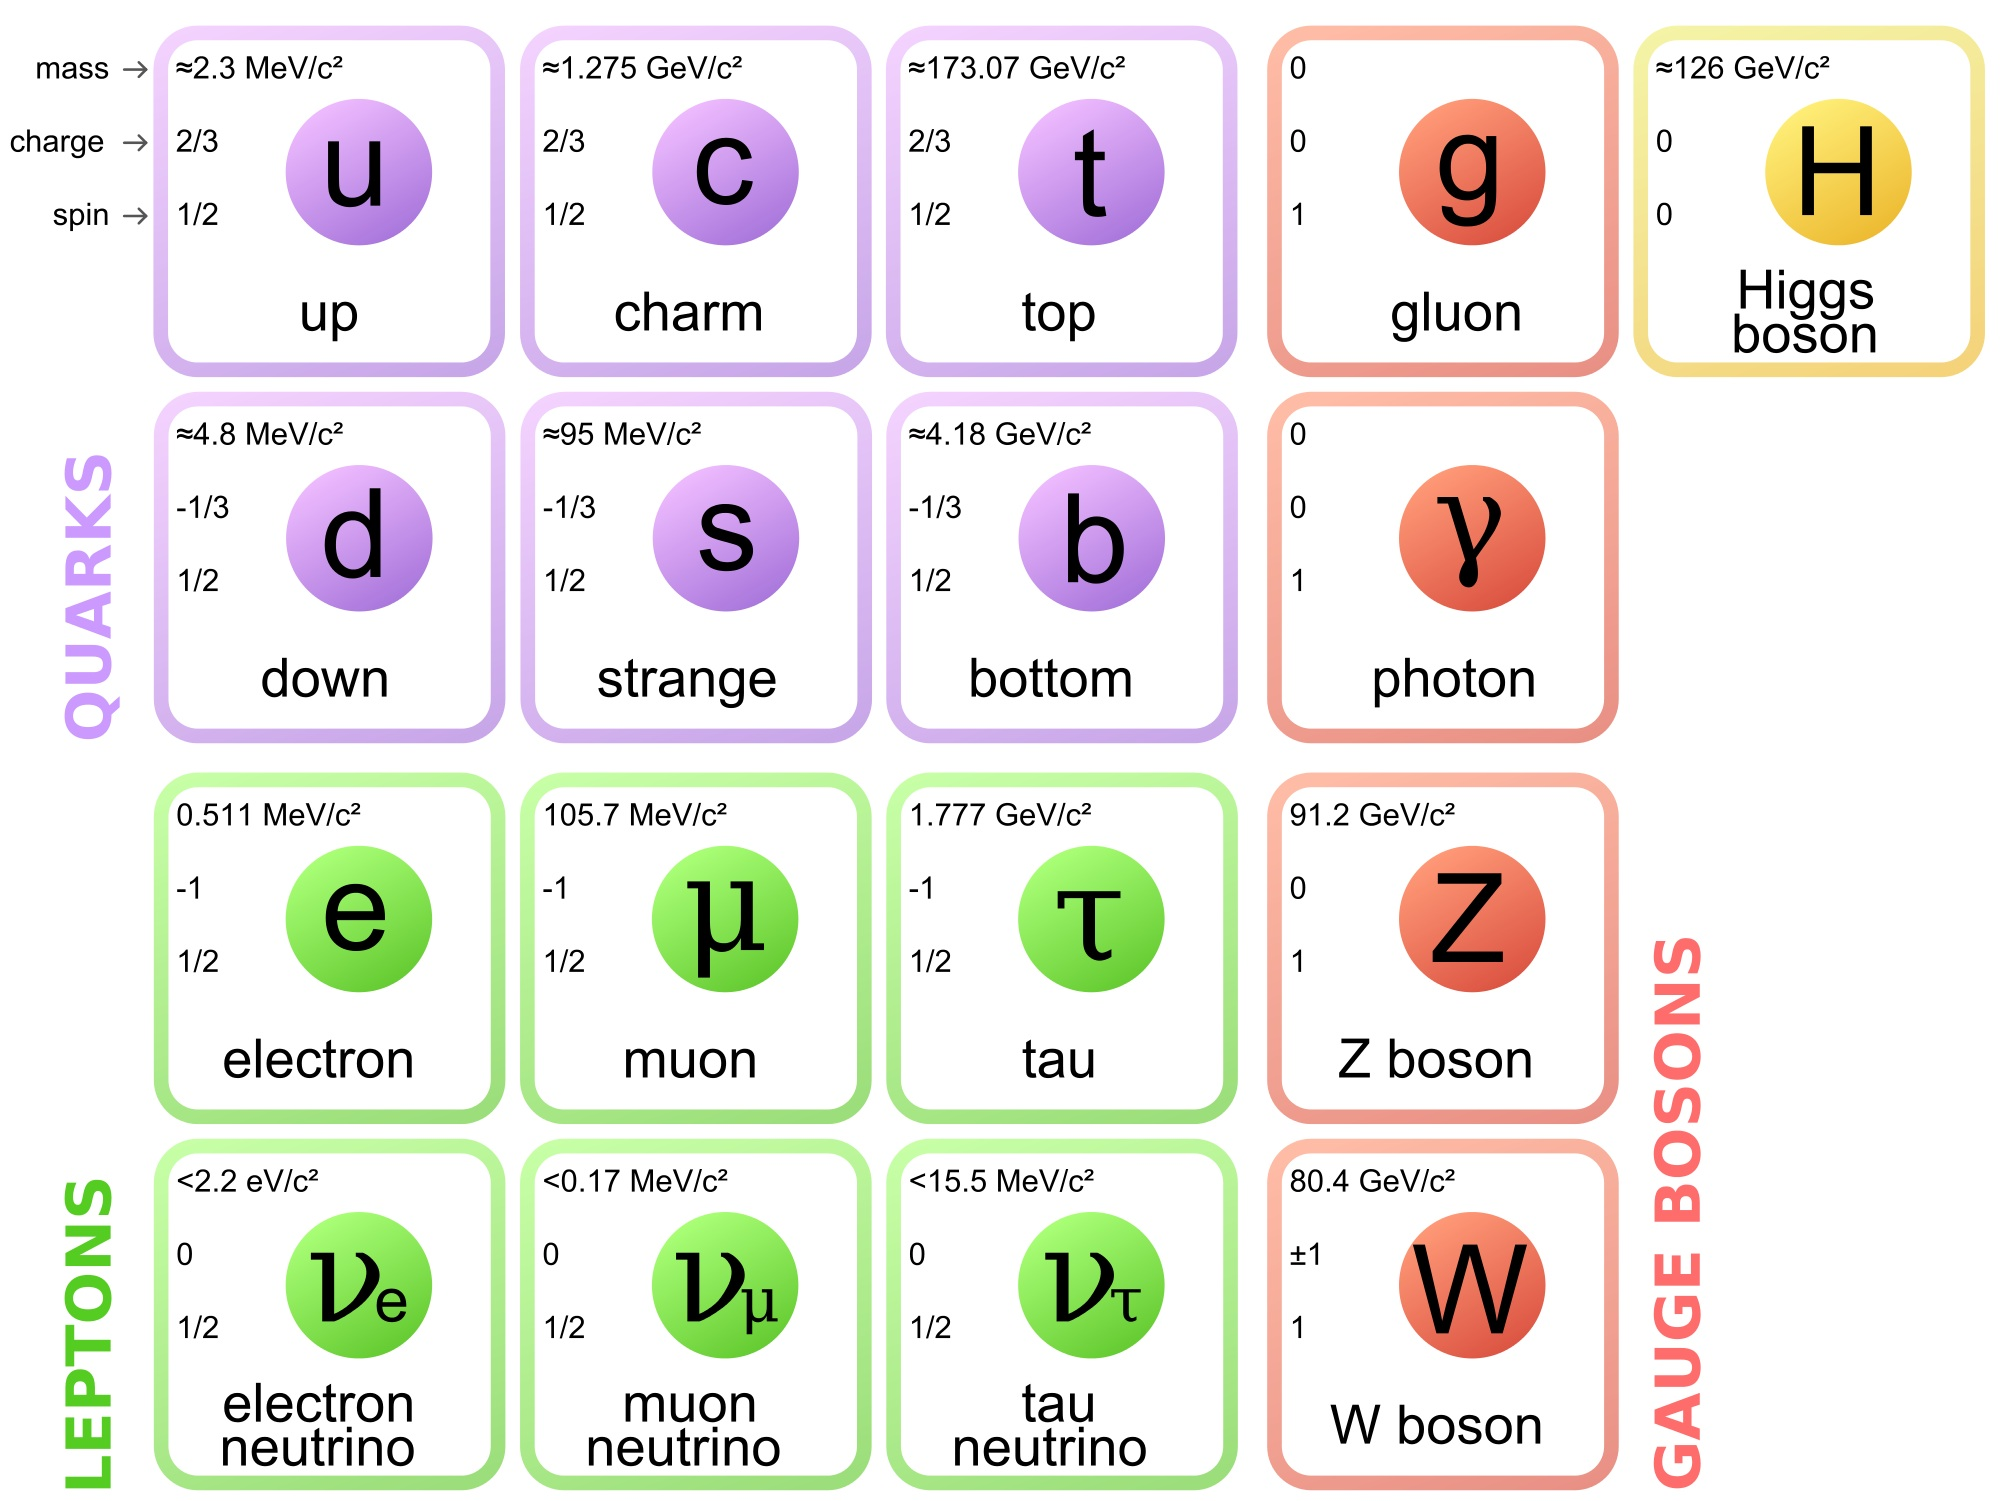
\includegraphics[width=.8\textwidth]{figures/theory/standard-model.jpg}
\caption{The particles of the Standard Model.}
\label{fig:sm}
\end{figure}

\subsection{Forces}



\paragraph{Leptons}
There are three generations of leptons, labeled by flavor, which interact via the electromagnetic and weak forces: electrons ($e$), muons ($\mu$), and taus ($\tau$), ordered by mass. Each lepton has negative electromagnetic charge and has an anti-particle with positive charge. There are also three generations of leptons which interact only via the weak force: electron neutrino ($\nu_{e}$), muon neutrino ($\nu_{\mu}$), and tau neutrinos ($\nu_{\tau}$), with unknown mass ordering. Neutrinos have no electromagnetic charge and tiny masses and thus are extremely hard to detect and not studied at the \ac{LHC}. In any \ac{SM} process, the number of leptons of each flavor is conserved. 

\subsection{Quarks}
There are three generations of quarks that interact via the electromagnetic, weak, and strong forces. Quarks are further divided into up-type with charge $+\frac{2}{3}q_{e}$ and down-type (with charge $-\frac{1}{3}q_{e}$). The up-type quarks are up ($u$), strange ($s$), and bottom ($b$), the down-type quarks are down ($d$), charm ($c$) and top ($t$). Since they also interact via the strong force, each quark also has a color charge, either red, blue, or green (or the opposite (anticolor)). Individual quarks are not seen in nature and all stable particles are color neutral with whole number charges, either a mix of all three colors or color and anticolor. In nature, quarks are found in color-neutral composite particles called \emph{hadrons}. Color-anticolor pairs are called \emph{mesons} and states with all three colors are called \emph{baryons}. The lightest hadron, the proton ($udd$), is stable, but all others are unstable and many are produced and decay at the \ac{LHC}.

Quarks formed at the \ac{LHC} hadronize due to the exponential coupling of the strong forces


\subsection{Gauge Bosons}


\subsection{Higgs Boson}


\section{Open Questions}
\section{Supersymmetry}

\section{GMSB}

\section{Simplified Models}

\section{Current Limits on Long Lived Sleptons}



